\documentclass[10pt,pdf,utf8,russian,aspectratio=169]{beamer}
\usepackage{cmap}
\usepackage[russian,english]{babel}
\usepackage[T2A]{fontenc}
\usepackage{subfig}
\usepackage{graphicx}
\usepackage{multicol}
\usepackage{cancel}
\usepackage{tabularx}
%
% Choose how your presentation looks.
%
% For more themes, color themes and font themes, see:
% http://deic.uab.es/~iblanes/beamer_gallery/index_by_theme.html
%
\mode<presentation>
{
  \usetheme{Boadilla}      % or try Darmstadt, Madrid, Warsaw, ...
  \usecolortheme{seagull} % or try albatross, beaver, crane, ..

  \usefonttheme{structurebold}  % or try serif, structurebold, ...
  \setbeamertemplate{navigation symbols}{}
  \setbeamertemplate{caption}[numbered]
} 

\captionsetup[subfloat]{labelformat=empty}
\title[Оптимизация гиперпараметров]{Оптимизация гиперпараметров}
\author{Бахтеев Олег}
\institute{МФТИ}
\date{23.10.2019}
%\renewcommand{\headrulewidth}{0pt}
\DeclareMathOperator*{\argmin}{arg\,min}
\DeclareMathOperator*{\argmax}{arg\,max}
\begin{document}

\begin{frame}
  \titlepage
\end{frame}

\begin{frame}{Что такое гиперпараметры}
\begin{block}{Определение}
Априорным распределением $p(\mathbf{w}|\mathbf{h})$ параметров модели назовем вероятностное распределение, соответствующее предположениям о
распределении параметров модели.
\end{block}

\begin{block}{Определение}
Гиперпараметрами $\mathbf{h} \in \mathbb{H}$ модели назовем параметры априорного распределения (параметры распределения параметров модели).
\end{block}

\end{frame}

\begin{frame}{Постановка задачи}
Задана дифференцируемая по параметрам модель, приближающая зависимую переменную~$y$:
\[
	\mathbf{f}:\mathbb{R}^n \to \mathbb{Y}, \quad \mathbf{w} \in \mathbb{R}^u.
\]
Функция $\mathbf{f}$ задает правдоподобие выборки $\text{log}p(\mathbf{y}|\mathbf{X}, \mathbf{w})$. 

Пусть также задано априорное распределение параметров $p(\mathbf{w}|\mathbf{h})$.
\vspace{1cm}
\textbf{Пример:}
 $$\mathbf{w} \sim \mathcal{N}(\mathbf{0}, \mathbf{A}^{-1}),$$
где $\mathbf{A}^{-1} = \text{diag}[\alpha_1, \dots, \alpha_u]^{-1}$ --- матрица ковариаций диагонального вида, определяемая \textit{гиперпараметрами} $[\alpha_1, \dots, \alpha_u] = \mathbf{h}$. 
\end{frame}

\begin{frame}{Постановка задачи}
Пусть $\boldsymbol{\theta} \in \mathbb{R}^s$ --- множество всех оптимизируемых параметров.\\
$L(\boldsymbol{\theta},\mathbf{h})$ ---  дифференцируемая функция потерь  по которой производится оптимизация функции $\mathbf{f}$. \\
$Q(\boldsymbol{\theta},\mathbf{h})$ ---  дифференцируемая функция определяющая итоговое качество модели $\mathbf{f}$ и приближающая интеграл.\\

Требуется найти параметры ${\boldsymbol{\theta}}^{*}$ и гиперпараметры ${\mathbf{h}}^{*}$ модели, доставляющие минимум следующему функционалу:
\[
{\mathbf{h}}^{*} = \argmax_{\mathbf{h} \in \mathbb{H}} Q({\boldsymbol{\theta}^{*}}(\mathbf{h}), \mathbf{h}),
\]
\[
	{\boldsymbol{\theta}}(\mathbf{h})^{*} =  \argmin_{\boldsymbol{\theta} \in \mathbb{R}^s} L(\boldsymbol{\theta}, \mathbf{h}).
\]
\end{frame}

\begin{frame}{Байесовский вывод}
Пусть $\boldsymbol{\theta} = [\mathbf{w}]^\mathsf{T}.$

\textit{Первый уровень:}
\[
{\boldsymbol{\theta}}^{*} = \argmax \bigl(-L(\boldsymbol{\theta}, \mathbf{h})\bigr) = p(\mathbf{w}|\mathbf{X}, \mathbf{y}, \mathbf{h}) = \frac{p(\mathbf{y}|\mathbf{X},\mathbf{w})p(\mathbf{w}|\mathbf{h})}{p(\mathbf{y}|\mathbf{X},\mathbf{h})}.
\]
\textit{Второй уровень:}
\[
p(\mathbf{h}|\mathbf{X}, \mathbf{y}) \propto p(\mathbf{y}|\mathbf{X},\mathbf{h})p(\mathbf{h}),
\]

Полагая распределение параметров $p(\mathbf{h})$ равномерным на некоторой большой окрестности, получим задачу оптимизации гиперпараметров:
\[
	Q(\boldsymbol{\theta}, \mathbf{h}) = p(\mathbf{y}|\mathbf{X},\mathbf{h}) = \int_{\mathbf{w} \in \mathbb{R}^u} p(\mathbf{y}|\mathbf{X}, \mathbf{w}) p(\mathbf{w}|\mathbf{h}) \to \max_{\mathbf{h} \in \mathbb{H}}.
\]
\end{frame}

\begin{frame}{Кросс-валидация}
Разобьем выборку $\mathfrak{D}$ на $k$ равных частей:
\[
\mathfrak{D} = \mathfrak{D}_1 \sqcup \dots \sqcup \mathfrak{D}_k.
\]


Запустим $k$ оптимизаций модели, каждую на своей части выборки. Положим $\boldsymbol{\theta} = [\mathbf{w}_1, \dots, \mathbf{w}_k]$, где $\mathbf{w}_1, \dots, \mathbf{w}_k$ --- параметры модели при оптимизации $k$.
 
Пусть $L$ --- функция потерь:
\begin{equation}
\label{eq:cv}
L(\boldsymbol{\theta}, \mathbf{h}) = -\frac{1}{k}\sum_{q=1}^k \bigl(\frac{k}{k-1}\text{log}p(\mathbf{y} \setminus \mathbf{y}_q|\mathbf{X}\setminus \mathbf{X}_q, \mathbf{w}_q) + \text{log}p(\mathbf{w}_q|\mathbf{h})\bigr).
\end{equation}

Пусть $Q$ --- функция качества модели:
\[
Q(\boldsymbol{\theta}, \mathbf{h}) = \frac{1}{k}\sum_{q=1}^k k\text{log}p(\mathbf{y}_q|\mathbf{X}_q, \mathbf{w}_q).
\]

\end{frame}






\begin{frame}{Вариационная нижняя оценка}
Пусть $L=-Q$:
\[
\label{eq:elbo}
\text{log}~p(\mathbf{y}|\mathbf{X},\mathbf{A})  
\geq 
\sum_{\mathbf{x},y} \text{log}~p({y}|\mathbf{x}, \hat{\mathbf{w}}) - D_\text{KL}\bigl(q (\mathbf{w}) || p (\mathbf{w}|\mathbf{A})\bigr) = -L(\boldsymbol{\theta}, \mathbf{A}^{-1}) = Q(\boldsymbol{\theta}, \mathbf{A}^{-1}),
\]
где $q$ --- нормальное распределение с диагональной матрицей ковариаций:
\[
\label{eq:diag}
	q \sim \mathcal{N}(\boldsymbol{\mu}_q, \mathbf{A}^{-1}_q),
\]
$$
D_\text{KL}\bigl(q (\mathbf{w}) || p (\mathbf{w}|\mathbf{f})\bigr) = \frac{1}{2} \bigl( \text{Tr} [\mathbf{A}\mathbf{A}^{-1}_q] + (\boldsymbol{\mu} - \boldsymbol{\mu}_q)^\mathsf{T}\mathbf{A}(\boldsymbol{\mu} - \boldsymbol{\mu}_q) - u +\text{ln}~|\mathbf{A}^{-1}| - \text{ln}~|\mathbf{A}_q^{-1}| \bigr).
$$

В качестве оптимизируемых параметров $\boldsymbol{\theta}$ выступают параметры распределения $q$:
\[
\boldsymbol{\theta} = [\alpha_1, \dots, \alpha_u, {\mu}_1,\dots,{\mu}_u].
\]

\end{frame}


\begin{frame}{Evidence vs Кросс-валидация}
Оценка Evidece:
\[
\text{log}~p(\mathfrak{D}|\mathbf{f}) = \text{log}~p(\mathfrak{D}_1|\mathbf{f}) + \text{log}~p(\mathfrak{D}_2|\mathfrak{D}_1, \mathbf{f}) + \dots +  \text{log}~p(\mathfrak{D}_n|\mathfrak{D}_1,\dots,\mathfrak{D}_{n-1}, \mathbf{f}).
\]

Оценка leave-one-out:
\[
\text{LOU} = \mathsf{E} \text{log}~p(\mathfrak{D}_n|\mathfrak{D}_1,\dots,\mathfrak{D}_{n-1}, \mathbf{f}).
\]

Кросс-валидация использует среднее значение последнего члена $p(\mathfrak{D}_n|\mathfrak{D}_1,\dots,\mathfrak{D}_{n-1}, \mathbf{f})$ для оценки сложности. \\
Evidence учитывает \textbf{полную} сложность описания заданной выборки, определяющую предсказательную способность модели с самого начала.
\end{frame}



\begin{frame}{Базовые методы оптимизации гиперпараметров}
Варианты:
\begin{itemize}
\item Поиск по решетке;
\item Случайный поиск.
\end{itemize}

Оба метода страдают от проклятия размерности.

Случайный поиск может быть более эффективным, если пространство гиперпараметров вырождено.
\begin{figure}
\begin{centering}
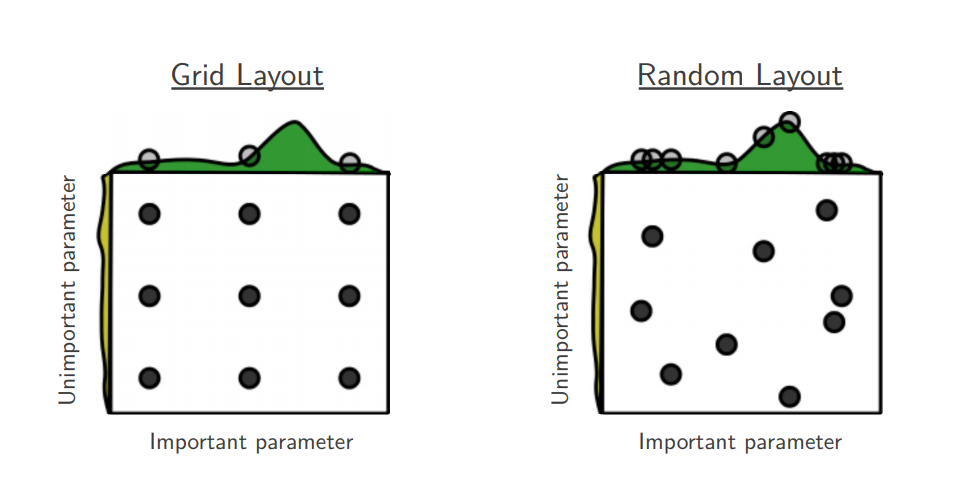
\includegraphics[width=0.5\textwidth]{random_search.png}
\end{centering}
\caption*{Bergstra et al., 2012}
\end{figure}
\end{frame}

\begin{frame}{Гауссовый процесс}

\begin{columns}
\begin{column}{0.5\textwidth}
\textbf{Идея:}

Будем моделировать $Q(\boldsymbol{\theta}(\mathbf{h})^{*}, \mathbf{h})$ гауссовым процессом, зависящим от $\mathbf{h}$.

~\\
\textbf{Плюсы:}
\begin{itemize}
\item Гибкость модели.
\item Дешевле, чем обучения модели.
\end{itemize}

~\\
\textbf{Минусы:} кубическая сложность по количеству гиперпараметров.

\end{column}
\begin{column}{0.4\textwidth}
\begin{figure}[h]
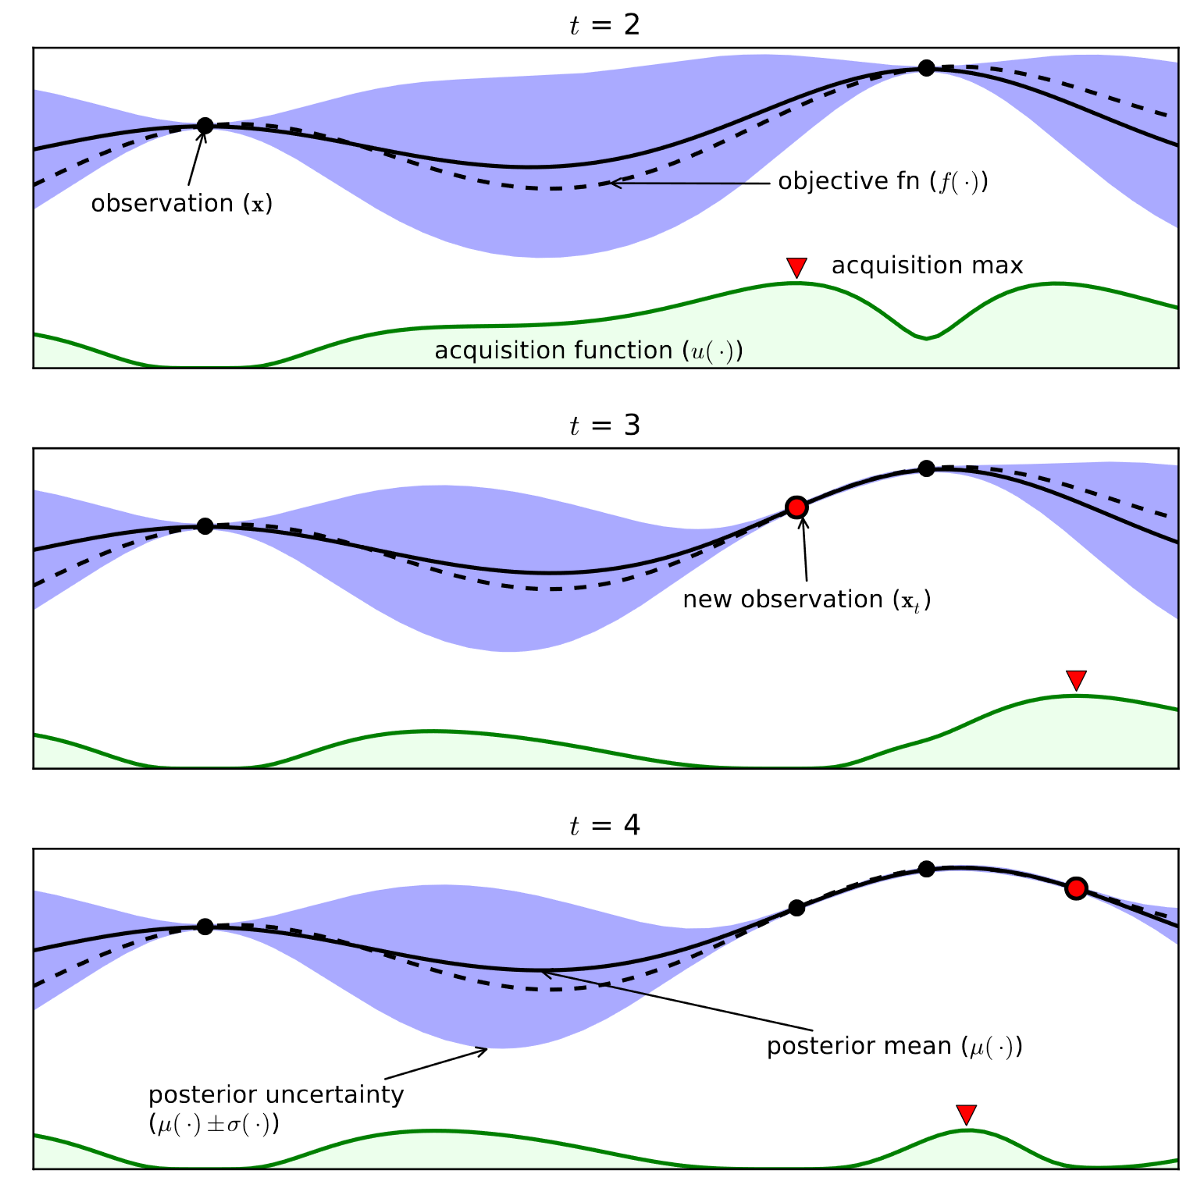
\includegraphics[width=\textwidth]{./gp.png}
\caption*{Shahriari et. al, 2016. Пример работы гауссового процесса.}
\end{figure}

\end{column}
\end{columns}
\end{frame}


\begin{frame}{Градиентные методы}
\begin{columns}
\begin{column}{0.5\textwidth}
\textbf{Идея:}
Будем производить оптимизацию вдоль всей траектории оптимизации параметров.

\textbf{Плюсы:}
\begin{itemize}
\item Оптимизация гиперпараметров будет учитывать оптимизацию параметров.
\item Сложность меняется незначительно от количества гиперпараметров.
\end{itemize}

~\\
\textbf{Минусы:} вычилсительно дорого.

\end{column}
\begin{column}{0.4\textwidth}
\begin{figure}[h]
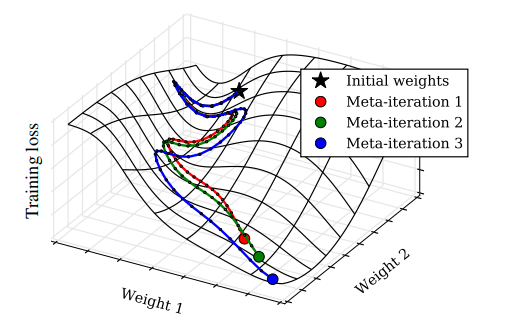
\includegraphics[width=\textwidth]{./grad.png}
\caption*{Maclaurin et. al, 2015. Пример работы.}
\end{figure}

\end{column}
\end{columns}

\end{frame}

\begin{frame}{Формальная постановка задачи: градиентная оптимизация}
\begin{block}{Определение}
Оператором $T$ назовем оператор стохастического градиентного спуска, производящий $\eta$ шагов оптимизации:
\begin{equation}
\label{eq:gd}
	 \hat{\boldsymbol{\theta}} = T \circ T \circ \dots \circ T(\boldsymbol{\theta}_0, \mathbf{h}) = T^\eta(\boldsymbol{\theta}_0, \mathbf{h}),
\end{equation}
где 
$$
	T(\boldsymbol{\theta}, \mathbf{h}) =\boldsymbol{\theta} - \beta \nabla L(\boldsymbol{\theta}, \mathbf{h})|_{\hat{\mathfrak{D}}}, 
$$
$\gamma$ --- длина шага градиентного спуска, $\boldsymbol{\theta}_0$ --- начальное значение параметров $\boldsymbol{\theta}$, $\hat{\mathfrak{D}}$ --- случайная подвыборка исходной выборки $\mathfrak{D}$.
\end{block}


Перепишем итоговую задачу оптимизации:
\[
	{\mathbf{h}}^{*} = \argmax_{\mathbf{h} \in \mathbb{H}} Q( T^\eta(\boldsymbol{\theta}_0, \mathbf{h})),
\]
где $\boldsymbol{\theta}_0$ --- начальное значение параметров $\boldsymbol{\theta}$.


\end{frame}

\begin{frame}{Forward-mode differentiation}
Идея дифференцирования: применение формулы:
\[
    \frac{\partial{y}}{\partial{x}}  = \frac{\partial{y}}{\partial{w_{n-1}}}\frac{\partial{w_{n-1}}}{\partial{x}} = \frac{\partial{y}}{\partial{w_{n-1}}}\left(\frac{\partial{w_{n-1}}}{\partial{w_{n-2}}}\frac{\partial{w_{n-2}}}x{\partial{x}}\right) = \dots. 
\]

Пример (wiki):
\[
x_1x_2 + \text{sin}(x_1)
\]
\begin{figure}
\centering
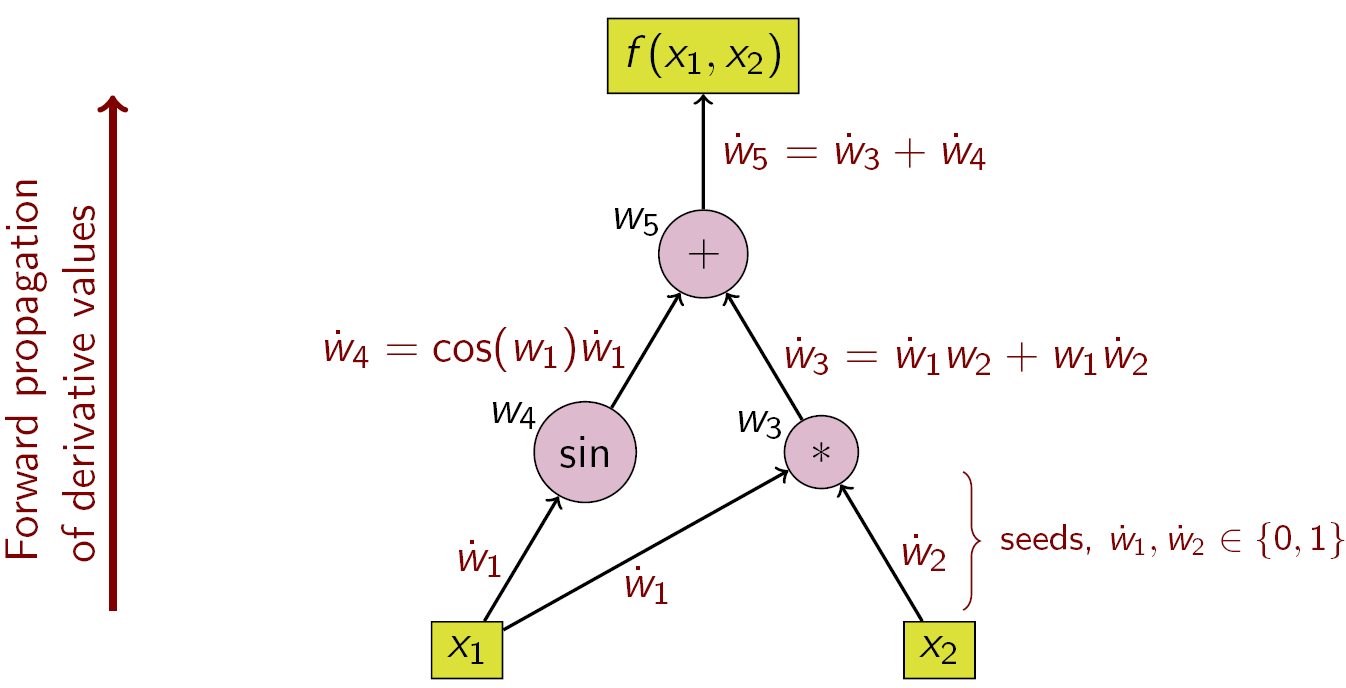
\includegraphics[width=0.5\textwidth]{fwd.png}
\end{figure}
\end{frame}


\begin{frame}{Reverse-mode differentiation}
Идея дифференцирования: применение формулы:
\[
    \frac{\partial{y}}{\partial{x}}  = \frac{\partial{y}}{\partial{w_1}}\frac{\partial{w_1}}{\partial{x}} = \left(\frac{\partial{y}}{\partial{w_2}}\frac{\partial{w_2}}{\partial{w_1}}\right)\frac{\partial{w_1}}{\partial{x}} = \dots. 
\]

\begin{figure}
\centering
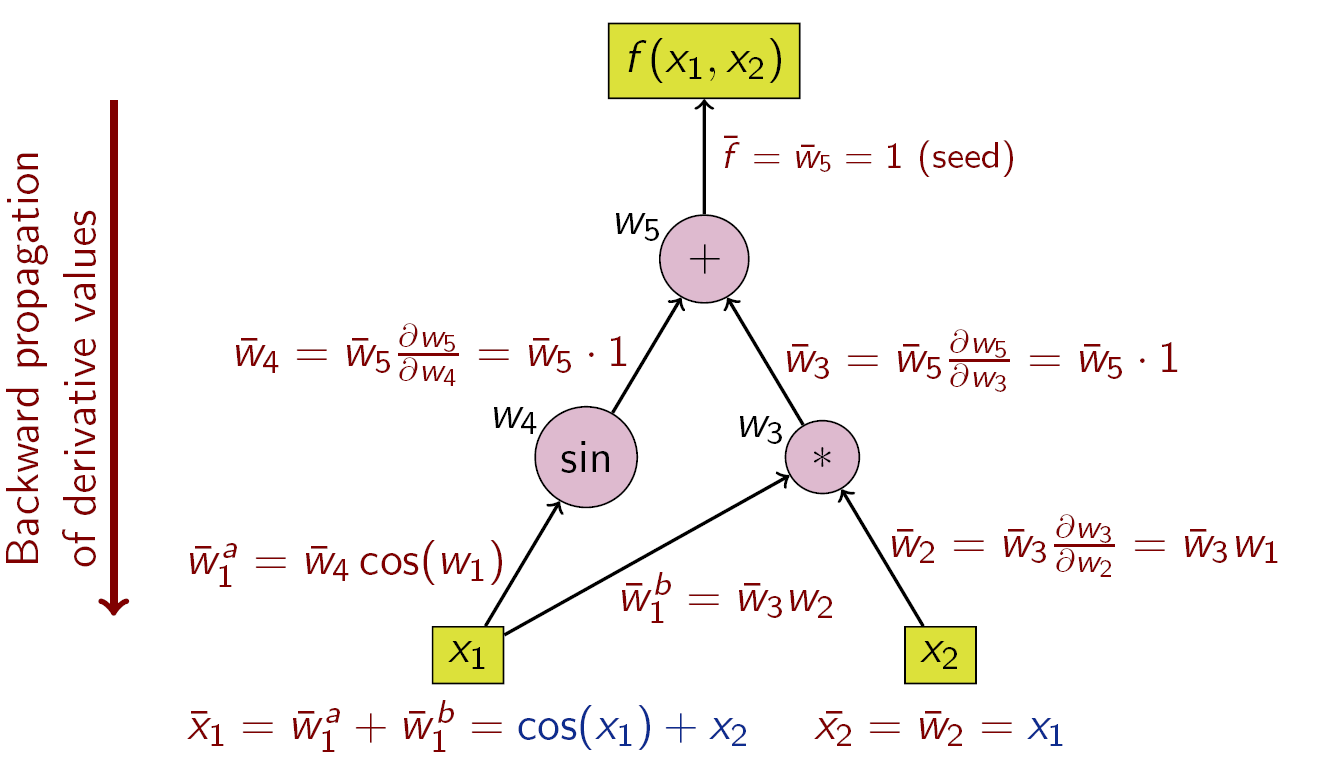
\includegraphics[width=0.5\textwidth]{rmd.png}
\end{figure}
\end{frame}


\begin{frame}{RMAD, Maclaurin et. al, 2015 }
\begin{columns}
\begin{column}{0.5\textwidth}
\begin{enumerate}
\item Провести $\eta$ шагов оптимизации с моментом $\gamma$: $\boldsymbol{\theta} = T(\boldsymbol{\theta}_0, \mathbf{h})$.
\item Положим $\hat{\nabla} \mathbf{h} = \nabla_\mathbf{h} Q(\boldsymbol{\theta}, \mathbf{h}).$ 
\item Положим $d\mathbf{v} = \mathbf{0}.$
\item Для $\tau = \eta \dots 1 $ повторить:
\item \quad Вычислить $\boldsymbol{\theta}^{\tau-1}$.
\item \quad Вычислить градиент на шаге $\tau-1$, используя RMD.
\end{enumerate}
\end{column}


\begin{column}{0.5\textwidth}
Алгоритм RMAD основывается на Reverse-mode differentiation.
\begin{figure}
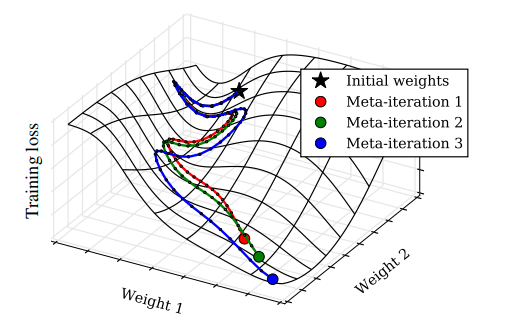
\includegraphics[width=\textwidth]{grad.png}
\end{figure}
\end{column}
\end{columns}
\end{frame}



\begin{frame}{DrMAD}
Алгоритм DrMad --- упрощенный RMAD. 
Вводится предположение о линейности траектории обновления параметров $\boldsymbol{\theta}$.
\begin{columns}
\begin{column}{0.5\textwidth}
\begin{enumerate}
\item Провести $\eta$ шагов оптимизации с моментом $\gamma$: $\boldsymbol{\theta} = T(\boldsymbol{\theta}_0, \mathbf{h})$.
\item Положим $\hat{\nabla} \mathbf{h} = \nabla_\mathbf{h} Q(\boldsymbol{\theta}, \mathbf{h}).$ 
\item Положим $d\mathbf{v} = \mathbf{0}.$
\item Для $\tau = \eta \dots 1 $ повторить:
\item \quad Вычислить $\boldsymbol{\theta}^{\tau-1}$.
\item \quad Вычислить градиент на шаге $\tau-1$, используя RMD.
\end{enumerate}
\end{column}
\begin{column}{0.5\textwidth}
\begin{enumerate}
\item Провести $\eta$ шагов оптимизации с моментом $\gamma$: $\boldsymbol{\theta} = T(\boldsymbol{\theta}_0, \mathbf{h})$.
\item Положим $\hat{\nabla} \mathbf{h} = \nabla_\mathbf{h} Q(\boldsymbol{\theta}, \mathbf{h}).$ 
\item Положим $d\mathbf{v} = \mathbf{0}.$
\item Для $\tau = \eta \dots 1 $ повторить:
\item $\boldsymbol{\theta}^{\tau-1} = \boldsymbol{\theta}_0 + \frac{\tau-1}{\eta} \boldsymbol{\theta}^{\eta}.$
\item \quad Вычислить градиент на шаге $\tau-1$, используя RMD.
\end{enumerate}

\end{column}
\end{columns}
\end{frame}



\begin{frame}{Аналитическая формула оптимизации параметров}
\begin{block}{Утверждение (Pedregosa, 2016)}
Пусть $L$ --- дифференцируемая функция, такая что все стационарные точки $L$ являются локальными минимумами.
Пусть также гессиан $\mathbf{H}^{-1}$ функции потерь $L$ является обратимым в каждой стационарной точке.\\
Тогда
\[
\nabla_{\mathbf{h}}Q(T(\boldsymbol{\theta}_0, \mathbf{h}), \mathbf{h}) =  \nabla_{\mathbf{h}}Q(\boldsymbol{\theta}^\eta, \mathbf{h}) - \nabla_{\mathbf{h}}\nabla_{\boldsymbol{\theta}} L(\boldsymbol{\theta}^\eta, \mathbf{h})^\text{T}\mathbf{H}^{-1}\nabla_{\boldsymbol{\theta}}Q(\boldsymbol{\theta}^\eta, \mathbf{h}).
\]
\end{block}
%\textbf{Схема доказательства}\\
%\begin{enumerate}
%\item Т.к. точка $\boldsymbol{\theta}^\eta$ стационарна, то $\nabla_{\boldsymbol{\theta}} L(\boldsymbol{\theta}^\eta, \mathbf{h}) = 0$.
%\item Продифференцируем выражение по $\mathbf{h}:$
%\[
%    \nabla_{\mathbf{h}}\nabla_{\boldsymbol{\theta}} L(\boldsymbol{\theta}^\eta, \mathbf{h} + \mathbf{h}\nabla_{\mathbf{h}}T(\boldsymbol{\theta}_0).
%\]
%\item По правилу дифференцирования сложной функции:
%\[
%\nabla_{\mathbf{h}}Q(T(\boldsymbol{\theta}_0), \mathbf{h}) =  \nabla_{\mathbf{h}}Q(\boldsymbol{\theta}^\eta, \mathbf{h})  + \nabla_{\mathbf{h}}T(\boldsymbol{\theta}_0)^%\text{T}\nabla_{\boldsymbol{\theta}}Q(\boldsymbol{\theta}^\eta, \mathbf{h}).
%\]
%\item Подставим в выражение 3 выражение 2 и получим искомое.
%\end{enumerate}
\end{frame}


\begin{frame}{Жадная оптимизация гиперпараметров}
На каждом шаге оптимизации параметров $\boldsymbol{\theta}$:
\[
	\mathbf{h}' = \mathbf{h} - \beta_{\mathbf{h}} \nabla_{\mathbf{h}}  Q \bigl(T(\boldsymbol{\theta}, \mathbf{h}) , \mathbf{h}\bigr) = \mathbf{h} - \beta_{\mathbf{h}} \nabla_{\mathbf{h}}  Q\bigl(\boldsymbol{\theta} - \beta \nabla L(\boldsymbol{\theta}, \mathbf{h}), \mathbf{h})\bigr),
\]
где $\beta_{\mathbf{h}}$ --- длина шага оптимизации гиперпараметров.

\begin{itemize}
\item Можно рассматривать как упрощение алгоритма RMAD, использующее только один элемент истории обновления параметров.
\item Является приближением к решению аналитической формуле в случае $\mathbf{H}^{-1} \sim \mathbf{I}$.
\end{itemize}

\end{frame}


\begin{frame}{HOAG}
Численное приближение аналитической формулы:
 \[\nabla_{\mathbf{h}}Q(\boldsymbol{\theta}^\eta, \mathbf{h}) - \nabla_{\mathbf{h}}\nabla_{\boldsymbol{\theta}} L(\boldsymbol{\theta}^\eta, \mathbf{h})^\text{T}\mathbf{H}^{-1}\nabla_{\boldsymbol{\theta}}Q(\boldsymbol{\theta}^\eta, \mathbf{h}).\]
\begin{enumerate}
\item Провести $\eta$ шагов оптимизации: $\boldsymbol{\theta} = T(\boldsymbol{\theta}_0, \mathbf{h})$.
\item Решить линейную систему для вектора $\boldsymbol{\lambda}$: $\mathbf{H}(\boldsymbol{\theta})\boldsymbol{\lambda} =  \nabla_{\boldsymbol{\theta}} Q(\boldsymbol{\theta}, \mathbf{h})$.
\item Приближенное значение градиентов гиперпараметра вычисляется как: $\hat{\nabla}_{\mathbf{h}}Q = \nabla_{\mathbf{h}}Q(\boldsymbol{\theta}, \mathbf{h}) -\nabla_{\boldsymbol{\theta}, \mathbf{h}} L(\boldsymbol{\theta}, \mathbf{h})^T\boldsymbol{\lambda}$.
\end{enumerate}

Итоговое правило обновления:
\[
\label{eq:update_hyper}
\mathbf{h}' = \mathbf{h} - \gamma_{\mathbf{h}} \hat{\nabla}_{\mathbf{h}}Q.
\]


\end{frame}

\begin{frame}{Сравнение алгоритмов}
\begin{table}
%\footnotesize
% Алгоритм & Тип алгоритм & Время & Плюсы & Минусы 

\begin{tabularx}{\textwidth}{|p{2cm}|X|X|}
\hline
\bf Алгоритм &  \bf + & \bf -  \\ \hline
Random search & Легко реализовать & Проклятие размерности  \\ \hline
Жадная оптимизация & Оптимизация проводится внутри цикла оптимизации параметров. Легко реализовать & Жадность, неоптимальность. \\ \hline
HOAG  & Быстрая сходимость.  & Качество результатов зависит от решения линейного уравнения $\mathbf{H}(\boldsymbol{\theta})\boldsymbol{\lambda} =  \nabla_{\boldsymbol{\theta}} Q(\boldsymbol{\theta}, \mathbf{h})$.\\ \hline 
DrMAD  & Учитывает особенности оператора оптимизации. Можно использовать для оптимизации мета-параметров.& Неустойчив при больших значениях длины градиентного шага $\gamma_\mathbf{h}$. Качество оптимизации зависит от кривизны траектории обновления параметров.\\ \hline
\end{tabularx}


\label{table:algo_descr}

\end{table}
\end{frame}

\begin{frame}
\begin{figure}  
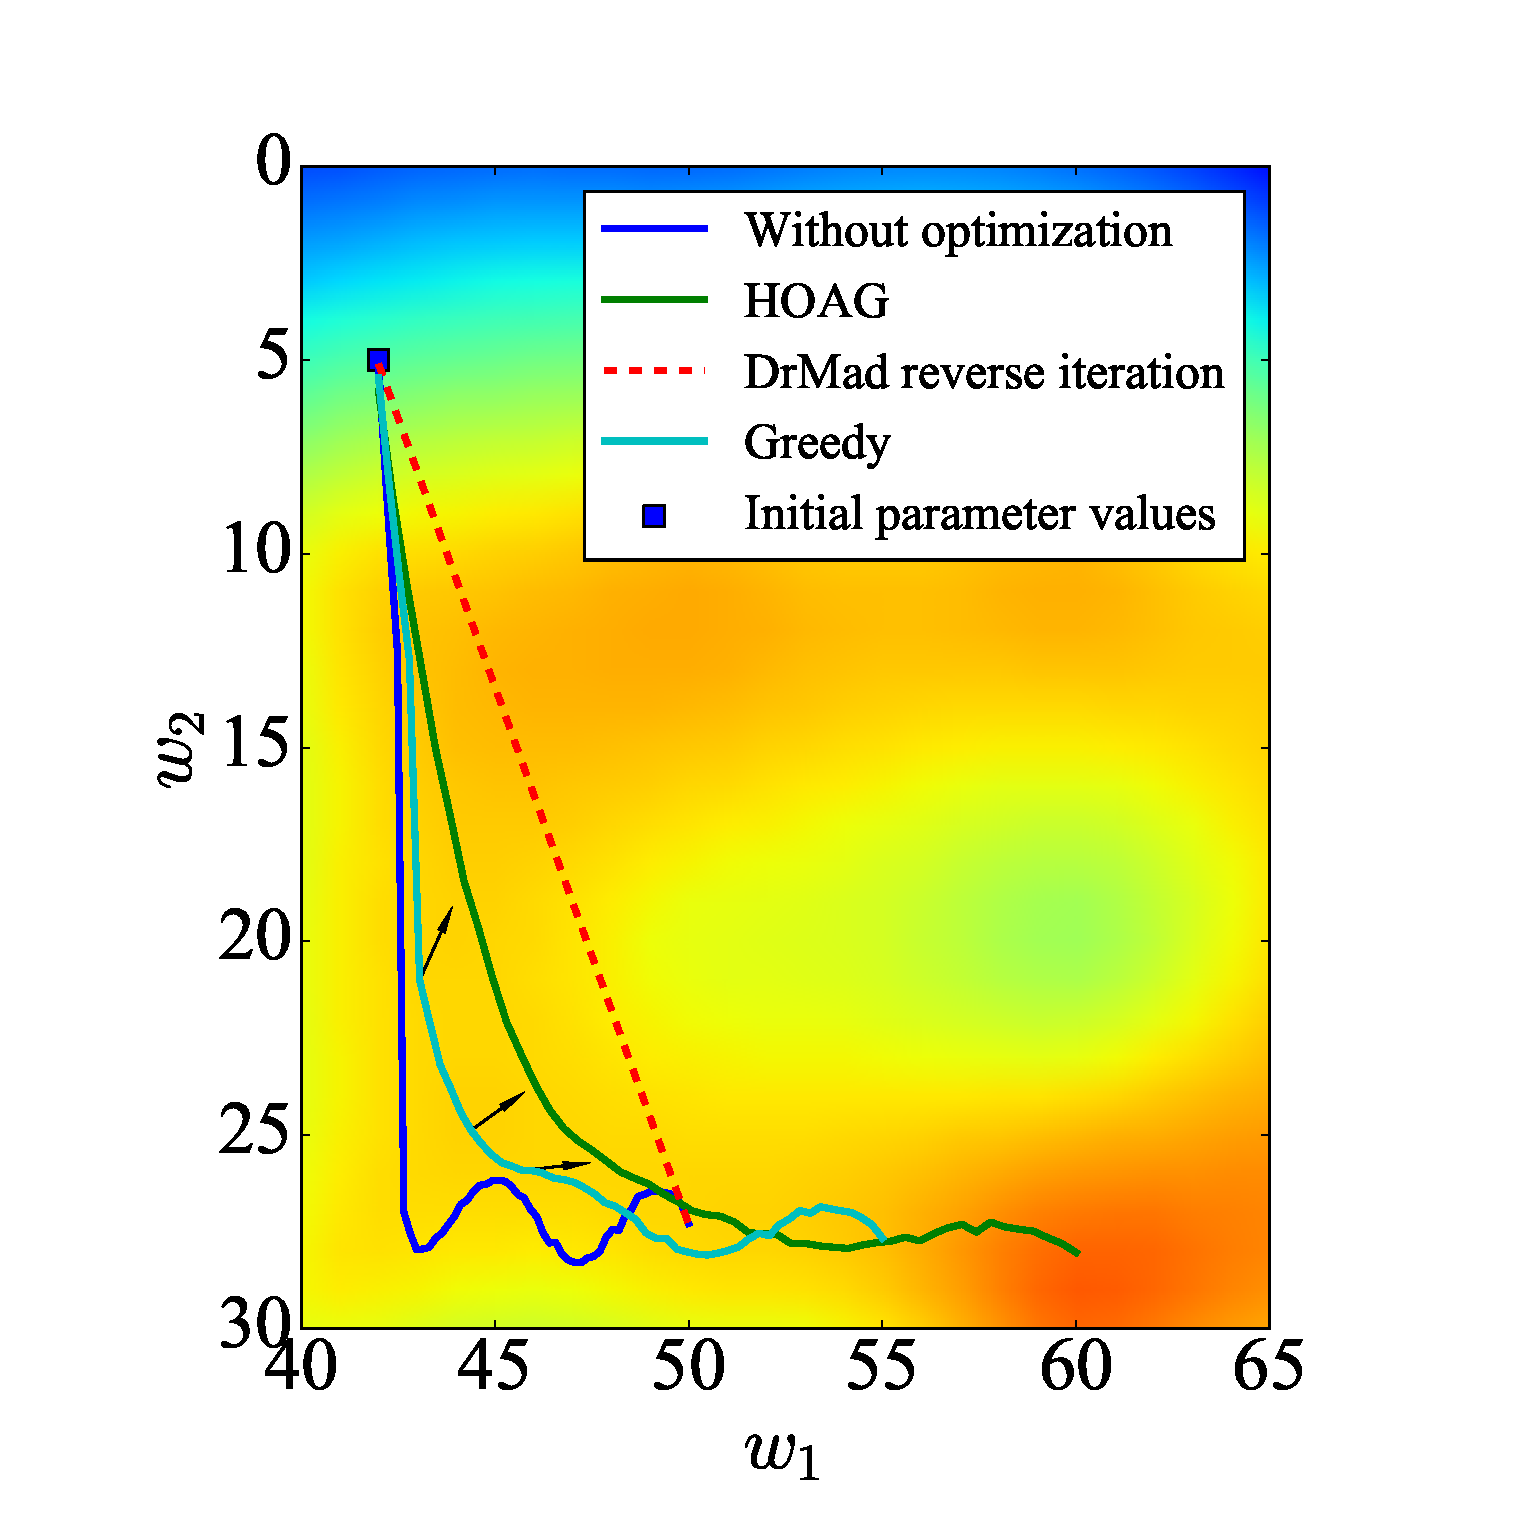
\includegraphics[width=0.5\textwidth]{Fig_traj.eps}
\end{figure}
\end{frame}

\begin{frame}{Эксперименты: полиномы}
\begin{figure}
  \centering
  \subfloat[Кросс-валидация]{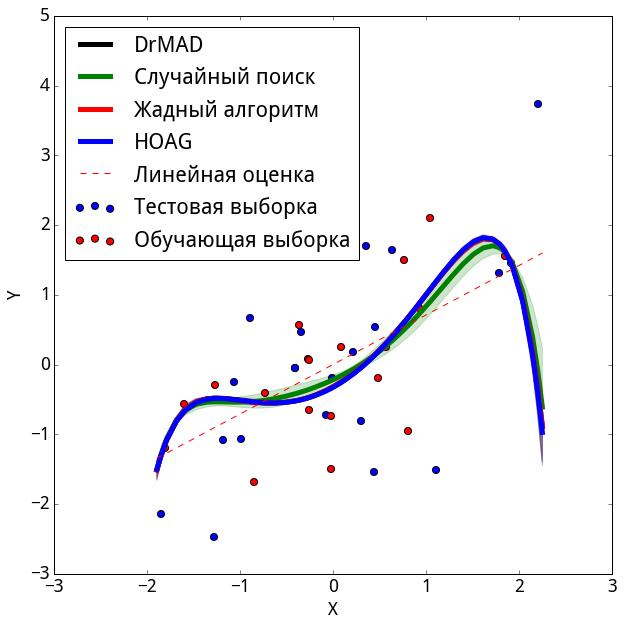
\includegraphics[width=0.42\textwidth]{poly_cv.png}} 
 \subfloat[Evidence]{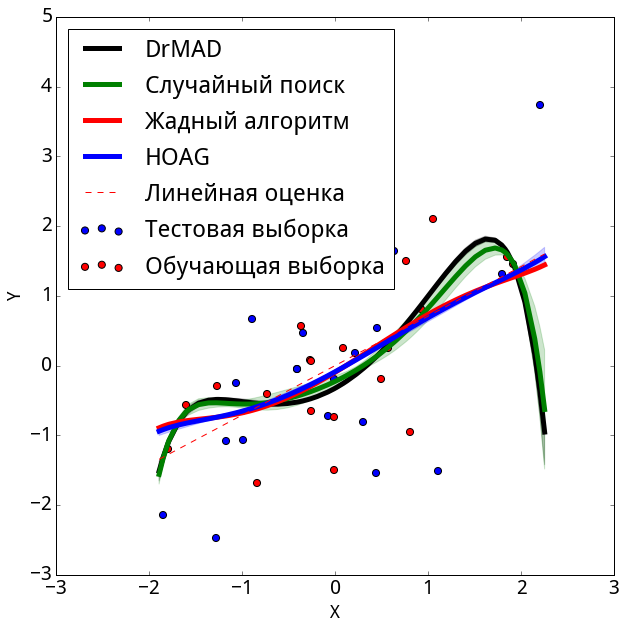
\includegraphics[width=0.42\textwidth]{poly_var.png}}
\label{fig:1}\qquad

\end{figure}
\end{frame}

\begin{frame}{Эксперименты: WISDM}
\begin{figure}  
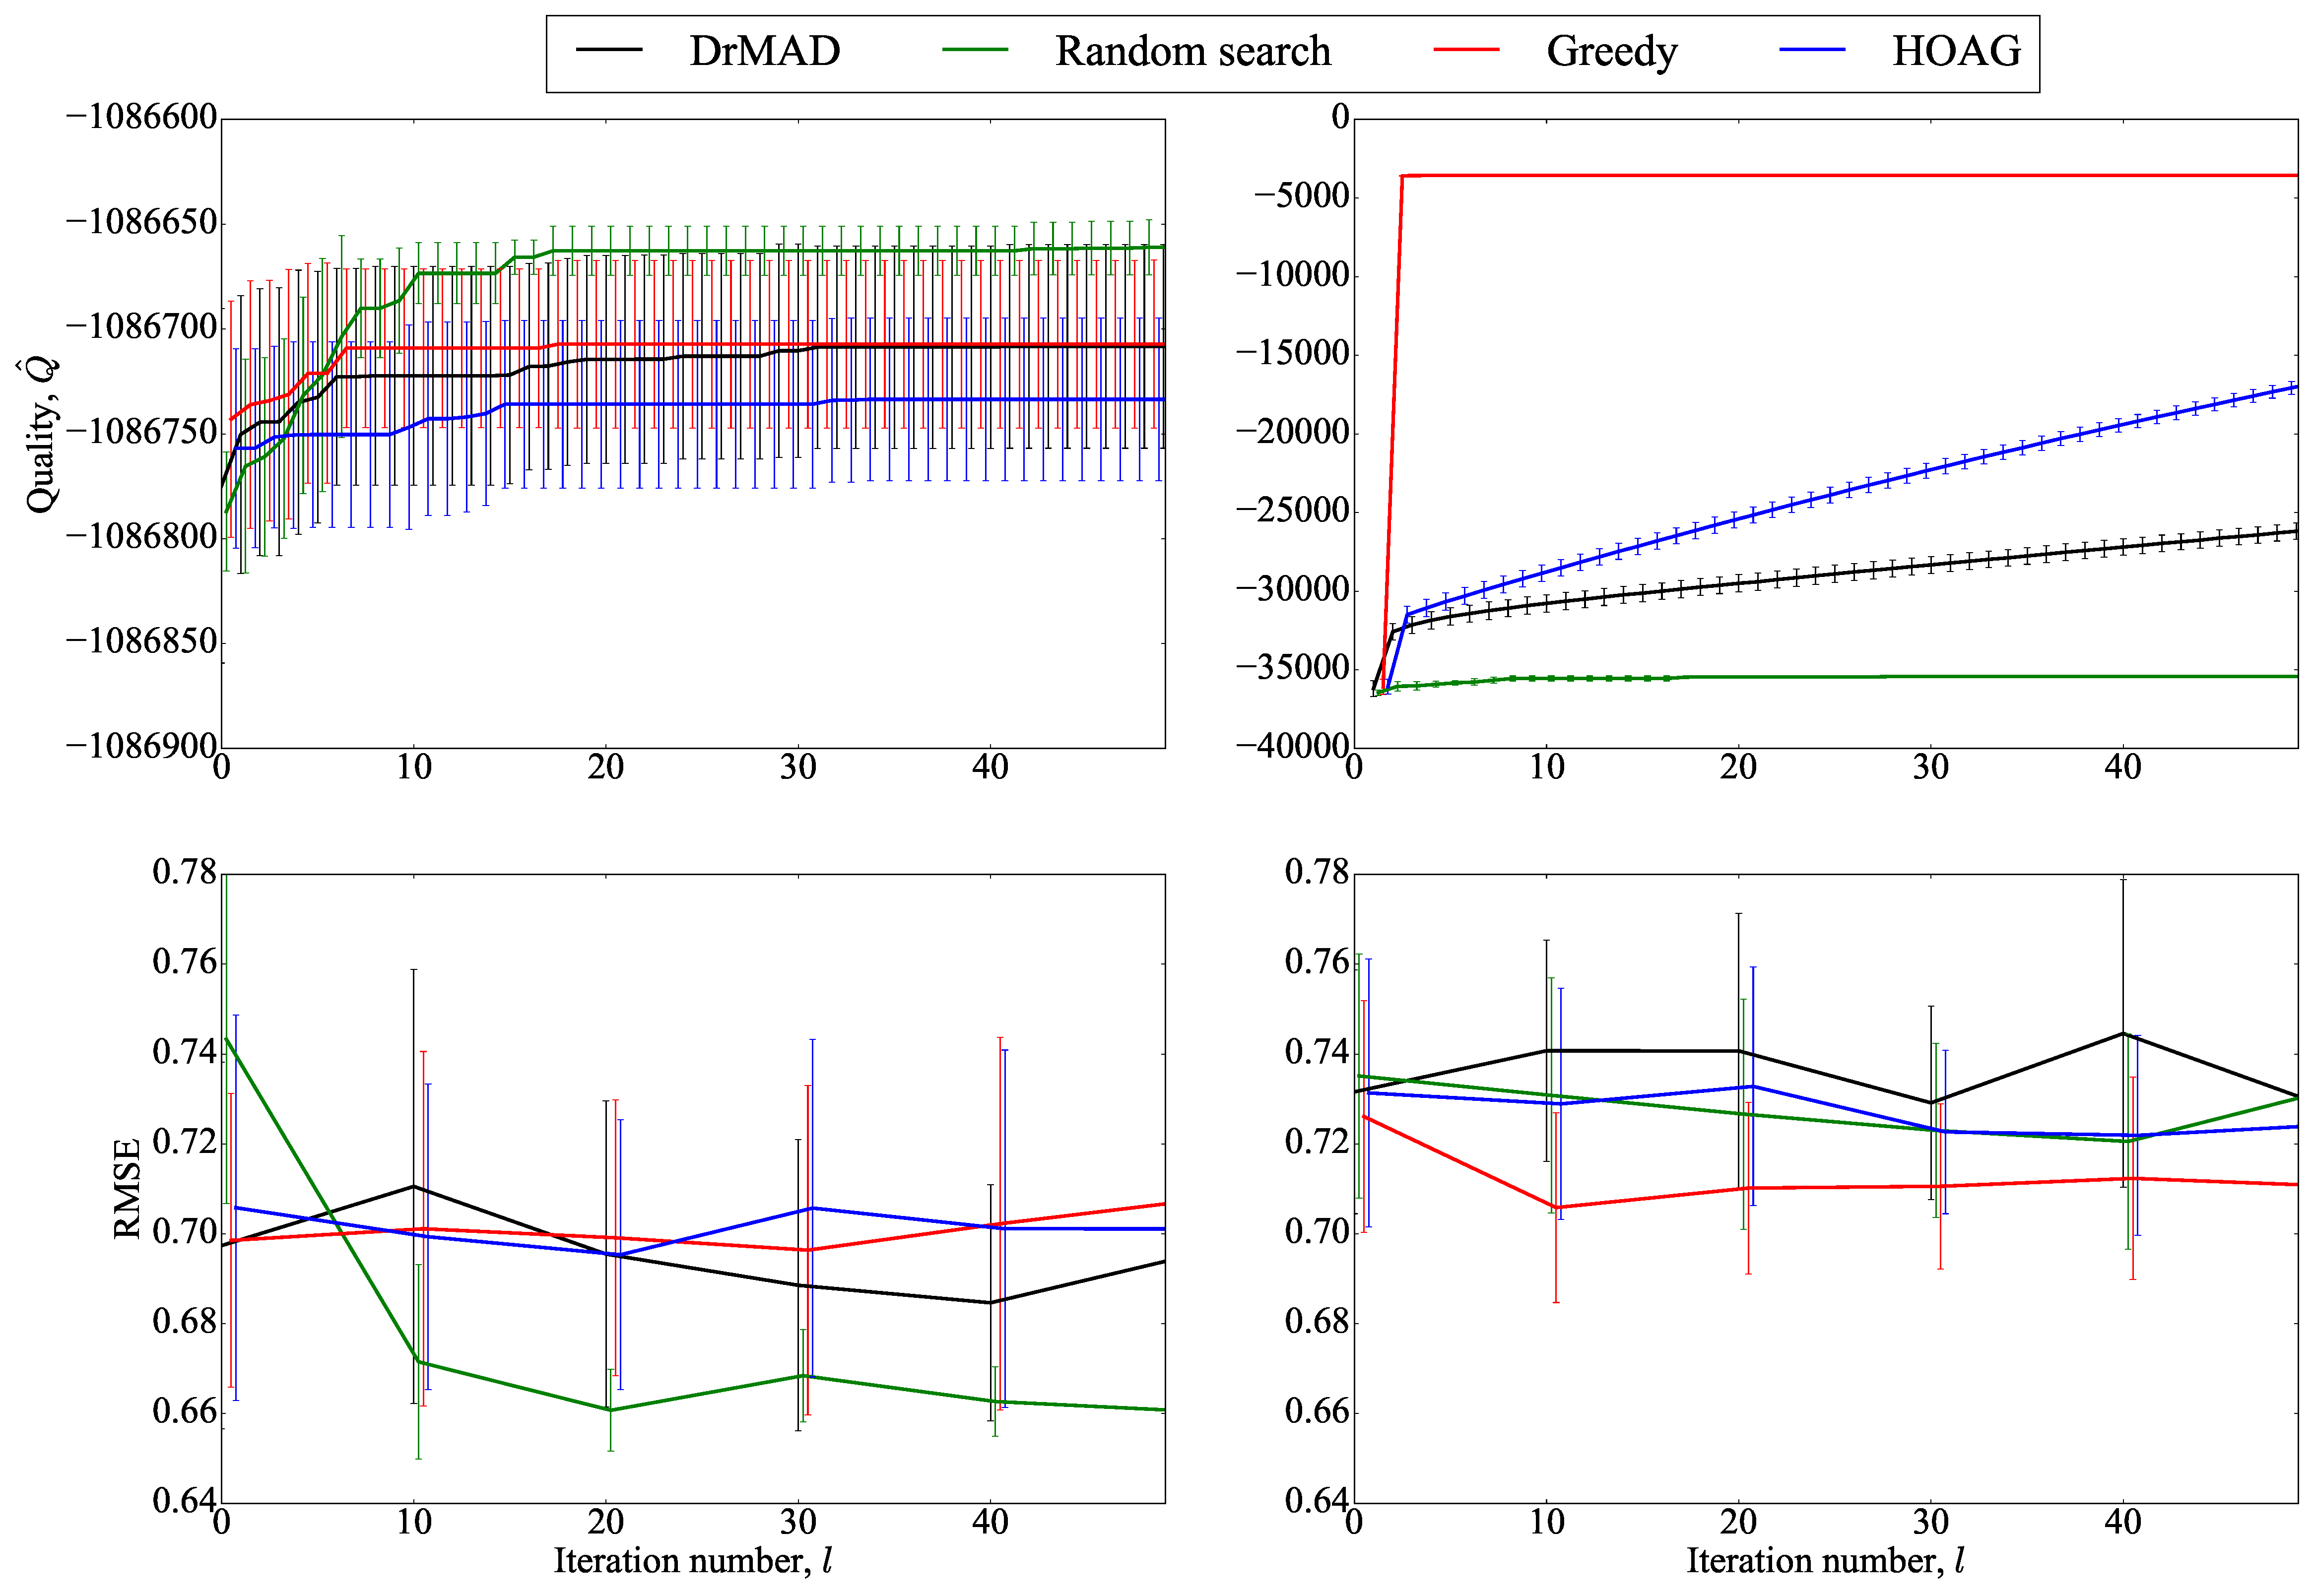
\includegraphics[width=0.7\textwidth]{Fig_wisdm.eps}
\end{figure}
\end{frame}

\begin{frame}{Эксперименты: MNIST}
\begin{figure}  
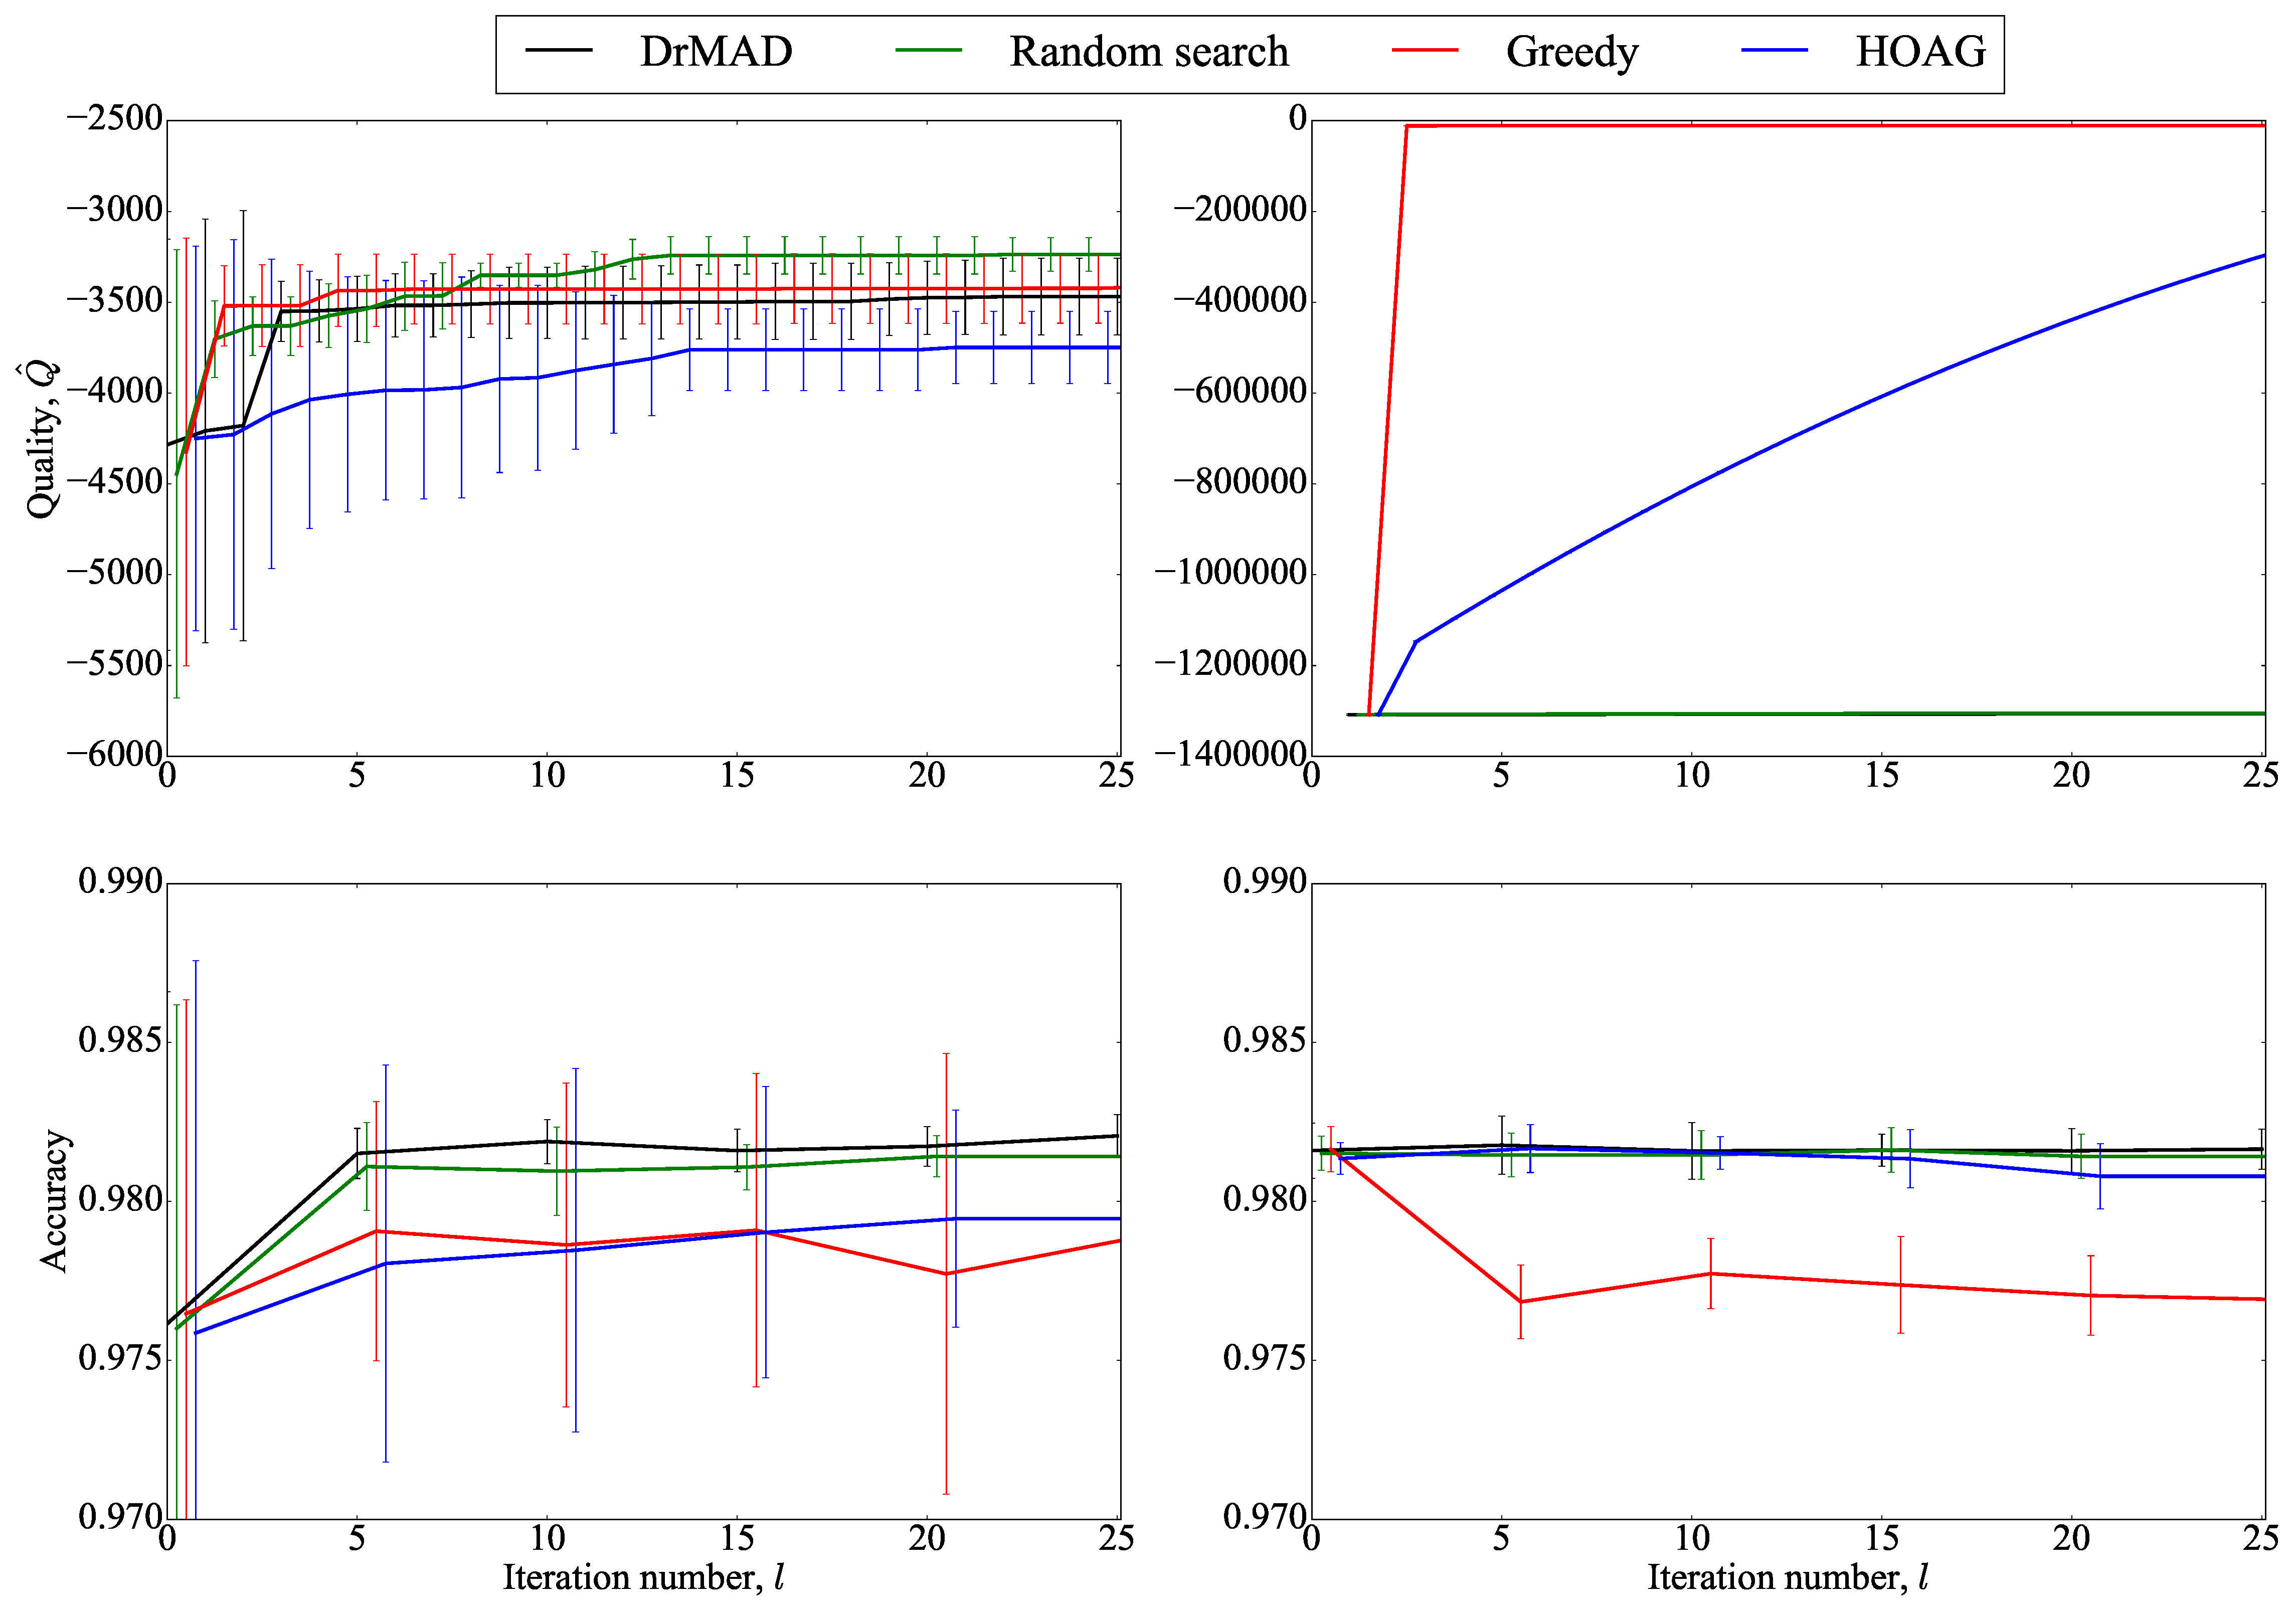
\includegraphics[width=0.7\textwidth]{Fig_mnist.eps}
\end{figure}
\end{frame}

\begin{frame}{Эксперименты: MNIST}
Добавление гауссового шума $\mathcal{N}(\mathbf{0},\sigma^2\mathbf{I})$:
\setlength{\columnsep}{10pt}
\begin{multicols}{4}
\begin{figure}[h]
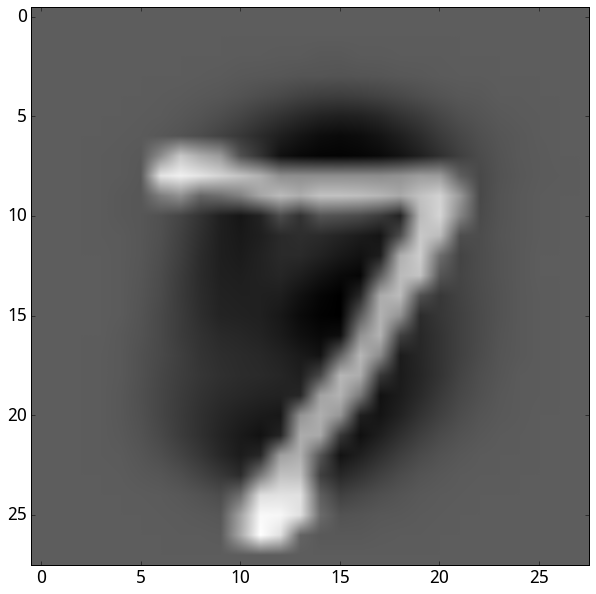
\includegraphics[width=0.10\textwidth]{./mnist0.png}
\caption*{Без шума}
\end{figure}

\begin{figure}[h]
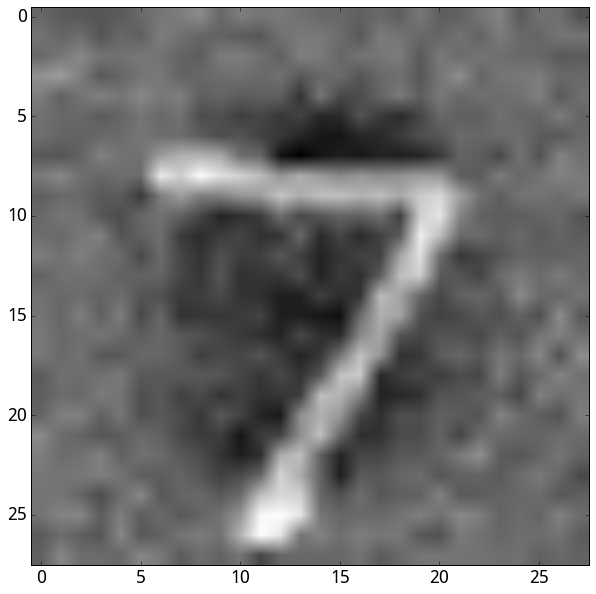
\includegraphics[width=0.08\textwidth]{./mnist10.png}
\caption*{$\sigma=0.1$}
\end{figure}

\begin{figure}[h]
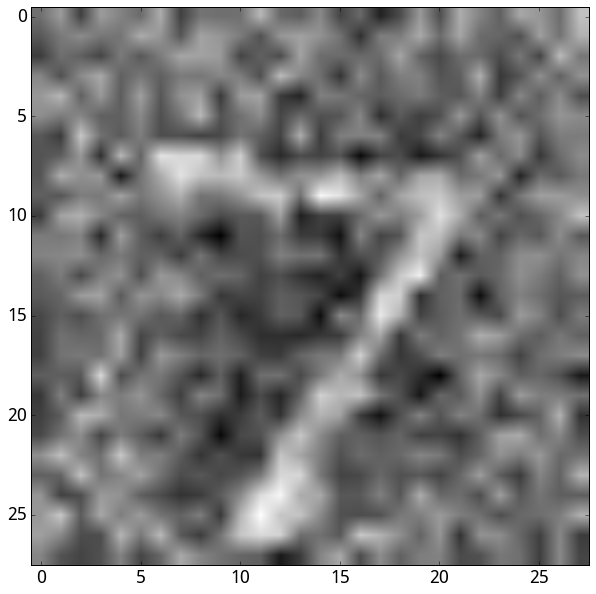
\includegraphics[width=0.08\textwidth]{./mnist25.png}
\caption*{$\sigma=0.25$}
\end{figure}

\begin{figure}[h]
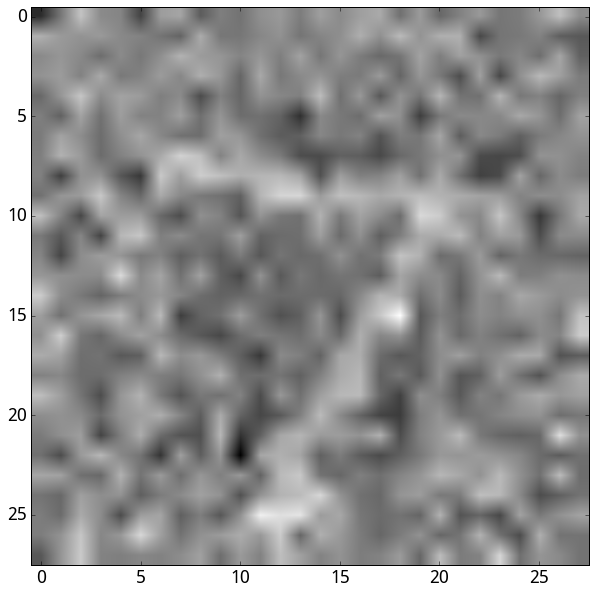
\includegraphics[width=0.08\textwidth]{./mnist50.png}
\caption*{$\sigma=0.5$}
\end{figure}
\end{multicols}
\begin{center}
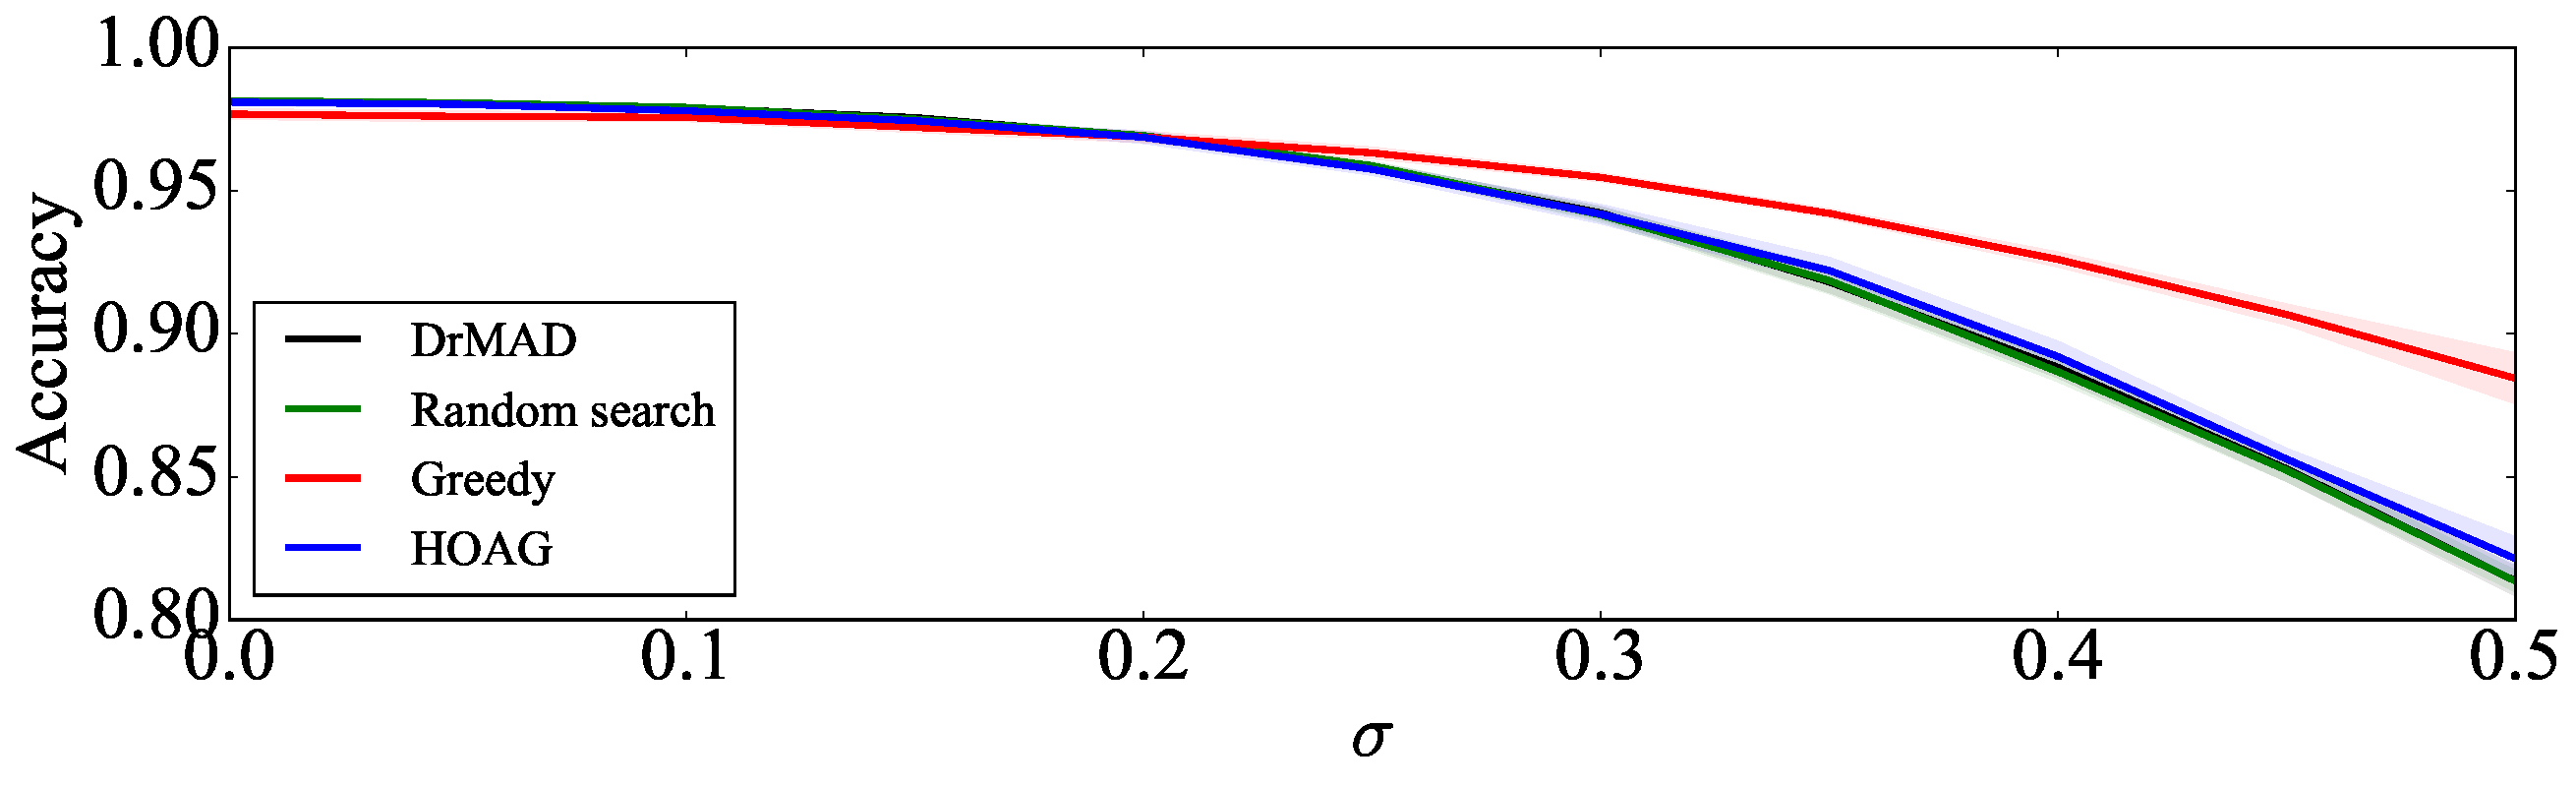
\includegraphics[width=0.85\textwidth]{Fig_noise.pdf}
\end{center}
\end{frame}

\begin{frame}{ДЗ: выбор задания}
\textbf{Дедлайн: 30 октября, 0 часов.}\\~\\

\texttt{ from zlib import crc32}\\~\\
\texttt{theory = crc32('фамилия кириллицей'.lower().encode('utf-8'))\%2+1}\\~\\
\texttt{practice = crc32('фамилия латиницей'.lower().encode('utf-8'))\%2+1}\\~\\

Задания заливаются на github:
\textit{https://github.com/Intelligent-Systems-Phystech/model\_selection/фамилия латиницей}\\

\end{frame}


\begin{frame}{ДЗ: теория}
\textbf{Формат: tex + pdf.}

\begin{enumerate}
\item Доказать утверждение (Pedregosa, 2016);
\begin{itemize}
\item Воспользоваться  (Pedregosa, 2016);
\end{itemize}

\item Расписать с комментариями RMAD для SGD без момента;
\begin{itemize}
\item Воспользоваться (Maclaurin et al., 2015).
\end{itemize}
\end{enumerate}
\end{frame}

\begin{frame}{ДЗ: практика}
\textbf{Формат: ipynb.}
Реализовать пример оптимизации гиперпараметров на небольшой выборке с ошибкой на валидации в качестве функции $Q$.

Количество гиперпараметров: не менее 20.

Рассмотреть алгоритмы: случайный поиск, гауссовый процесс (библиотечная реализация) и:
\begin{enumerate}
\item HOAG;

\item Жадный алгоритм.

\end{enumerate}

При оценивании будут учитываться аккуратность кода ноутбуков и наглядность примера.\\~\\
Пример должен быть выполнен на  \textbf{простых} игрушечных синтетических данных.
\end{frame}


\begin{frame}
\frametitle{Используемые материалы}
\begin{enumerate}
\item David J. C. MacKay, Information Theory, Inference \& Learning Algorithms, 2003
\item Christopher Bishop, Pattern Recognition and Machine Learning, 2006
\item Bergstra et al., Random Search for Hyper-Parameter Optimization, 2012
\item  Dougal Maclaurin et. al, Gradient-based Hyperparameter Optimization through Reversible Learning, 2015
\item Jelena Luketina et. al, Scalable Gradient-Based Tuning of
Continuous Regularization Hyperparameters, 2016
\item Jie Fu et. al, DrMAD: Distilling Reverse-Mode Automatic Differentiation for Optimizing
Hyperparameters of Deep Neural Networks, 2016
\item Fabian Pedregosa, Hyperparameter optimization with approximate gradient, 2016
\item Bobak Shahriari et. al,  Taking the Human Out of the Loop:
A Review of Bayesian Optimization, 2016
\item Bakhteev, Strijov, Comprehensive analysis of gradient-based hyperparameter optimization algorithms, 2018
\item Feurer et al, AUTOML: METHODS, SYSTEMS, CHALLENGES 
\end{enumerate}
\end{frame}
\end{document}
